\documentclass[beamer]{standalone}

\usetheme{naked}
\setbeamercolor{alerted text}{fg=green!50!black}
\setbeamercolor{box title}{fg=purple}
\setbeamertemplate{frametitle}{}

% \usepackage{xkeyval}
% \usepackage{pgffor}

\usepackage{standalone}

\makeatletter
../code-graphs.tex
\makeatother

% vertical centering of cells
% see http://tex.stackexchange.com/questions/46386/vertically-center-cells-of-a-table
\usepackage{array}% http://ctan.org/pkg/array
\newcolumntype{M}{>{\centering\arraybackslash}m{\dimexpr.17\linewidth-2\tabcolsep}}

% remove space between margin and lists
\usepackage{enumitem}
\setitemize{label=\usebeamerfont*{itemize item}%
  \usebeamercolor[fg]{itemize item}
  \usebeamertemplate{itemize item}}
\setlist{leftmargin=*,labelindent=0cm}

%\usepackage{amsmath}

\usepackage{tikz}
\usepackage{tkz-graph}
\usepackage{tkz-berge}
\usepackage{tkz-berge-add}

\usepackage[utf8]{inputenc}
% \usepackage{libertine}
% \usepackage[libertine]{newtxmath}

%\usepackage{lxfonts}

\usepackage{cabin}
\usepackage{mathastext}

\newcommand{\graphcaption}[4][gray!80!white]{\draw (#2,#3) node [fill=#1]{#4};}

\SetVertexSimple[FillColor=gray, MinSize=10pt, LineWidth=1.5pt]

\tikzset{EdgeStyle/.style= {%
    color           = white,
    double          = black,
    double distance = 2.5pt}}

\newcommand{\setof}[2]{\left\{\,#1\mid #2\,\right\}}

\newcommand{\triangulo}[4]{%
  \shadedraw[inner color=#4,opacity=0.8,line width=1pt]
  (#1.center) -- (#2.center) -- (#3.center) -- cycle;}

\newcommand{\triangleshaded}[3]{%
  \draw[fill=gray]
  (#1.center) -- (#2.center) -- (#3.center) -- cycle;}

\newcommand{\triang}[3]{%
  \shadedraw[inner color=gray,,opacity=0.8,line width=1pt]
  (#1.center) -- (#2.center) -- (#3.center) -- cycle;}

\begin{document}

\SetVertexSimple[FillColor=gray, MinSize=0.7pt, InnerSep=0.7pt, LineWidth=0.5pt]

\tikzset{EdgeStyle/.style= {%
    color           = white,
    double          = black,
    double distance = 0.5pt}}

\setlength{\fboxsep}{1pt}

\begin{standaloneframe}
    \begin{center}
    %\tiny
    \scriptsize
    \begin{tabular}{|M|M|}
      \hline
      $L$ & loc. $L$ \\
      \hline
      $K_{1}$ & $K_{2}$ \\
      $K_{2}$ & $K_{3}$ \\
      $K_{3}$ & $K_{4}$\\
      $C_{4}$ & $O_{3}$\\
      $K_{4}$ & $K_{5}$\\
      $C_{5}$ & icosaedro\\
      \graphst{i=25}{0.3} & \only<1>{$\overline{C_{8}}$} \only<2->{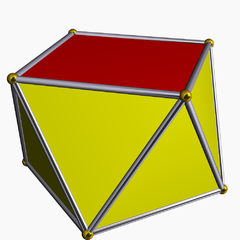
\includegraphics[width=0.6cm]{antiprism4}}\\
      $K_{5}$ & $K_{6}$\\
      \graphst{i=53}{0.3} & \only<1-2>{cubo chato} \only<3->{\includegraphics[width=0.6cm]{snubcube}}\\
      \hline
    \end{tabular}
    \begin{tabular}{|M|M|}
      \hline
      $L$ & loc. $L$ \\
      \hline
      \graphst{i=57}{0.3} & \only<1-3>{$L(O_{3})$} \only<4->{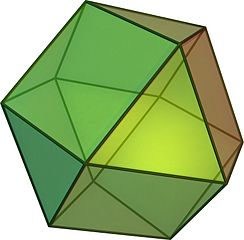
\includegraphics[width=0.6cm]{cuboctaedro}} \\
      \graphst{i=58}{0.3} & \only<1-4>{$L(K_{5})$} \only<5->{tipo de $\vee_{4} S^{2}$} \\
      \graphst{i=60}{0.3} & \only<1-5>{$C_{10}^{2,4}$} \only<6->{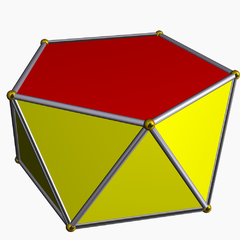
\includegraphics[width=0.6cm]{antiprism5}}\\
      $K_{3,3}$ & \only<1-6>{$K_{3,3,3}$} \only<7->{tipo de $\vee_{8} S^{2}$}\\
      \graphst{i=62}{0.2} & \only<1-7>{$\overline{C_{9}}$} \only<8->{tipo de $\vee_{2} S^{2}$} \\
      $O_{3}$ & $O_{4}$\\
      $K_{6}$ & $K_{7}$\\
      \hline
    \end{tabular}

    \bigskip
    \small

    Las extensiones únicas
  \end{center}
\end{standaloneframe}
\end{document}
